\documentclass[conference]{IEEEtran}
\usepackage{cite}
\usepackage{amsmath,amssymb,amsfonts}
\usepackage{algorithmic}
\usepackage{graphicx}
\usepackage{textcomp}
\usepackage{xcolor}
\usepackage{booktabs}
\usepackage{microtype}
\usepackage{url}

% Automatic image directory discovery
\graphicspath{{results/}{./results/}{./}}

\begin{document}

\title{Concurrent LSM-Tree Storage Engine: Lock-Free Writes with Fully Parallel Compaction}

\author{
    \IEEEauthorblockN{
        Aman Yadav (241AI004)\quad
        Shah Aagam Alpesh (241AI036)\quad
        Chhitanshu Shekhar (241AI012)\quad
        Harshvardhan Choudhary (241AI017)
    }
    \IEEEauthorblockA{
        \textit{Department of Information Technology} \\
        \textit{National Institute of Technology Karnataka, Surathkal}\\
        Srinivasnagar, Mangalore, India
    }
}

\maketitle

\begin{abstract}
Log-Structured Merge (LSM) Trees, employed in systems like Google Bigtable, LevelDB, RocksDB, and Apache Cassandra, are designed to convert random disk writes into high-throughput sequential operations. However, most textbook explanations and academic implementations describe LSM-Trees sequentially—where single writes execute in isolation and compaction pauses ingestion. In practice, making an LSM-Tree concurrent introduces significant synchronization challenges: coarse-grained locks on in-memory buffers cause severe contention, and single-threaded compaction routines trigger foreground write stalls. This project implements a concurrent C++17 LSM-Tree storage engine from scratch to study and benchmark these synchronization dynamics. Our engine combines a lock-free, CAS-based SkipList MemTable with a concurrent Write-Ahead Log (WAL) to allow multi-threaded writes without mutual exclusion, paired with an autonomous background compaction pool that merges disjoint SSTable key ranges concurrently using immutable snapshots. We evaluate our design across 1 to 32 threads against two foundational baselines: a single Global-Lock MemTable and a 16-Shard Partitioned MemTable under both Uniform and skewed Zipfian ($s=1.0$) access patterns. Experimental results demonstrate that while global locking collapses under high thread counts ($168.9$~K~ops/sec at 32 threads) and sharding bottlenecks under skewed access ($695.0$~K~ops/sec), our lock-free engine sustains scalable throughput up to $2.15$~M~ops/sec ($28.3$~$\mu$s P99 tail latency) under uniform workloads and $1.89$~M~ops/sec ($32.7$~$\mu$s P99 tail latency) under severe Zipfian skew at 32 threads, providing practical insights into synchronization overheads in concurrent storage engines.
\end{abstract}

\begin{IEEEkeywords}
Parallel Computing, LSM-Tree, Lock-Free SkipList, Compare-And-Swap, Parallel Compaction, Tail Latency, Storage Concurrency.
\end{IEEEkeywords}

\section{Introduction}
Modern write-intensive applications such as sensor networks, IoT telemetry pipelines, transaction ledgers, and real-time log aggregators require ingesting large volumes of updates within tight latency constraints. Writing data directly to secondary storage media (such as SSDs or HDDs) is slow. If a database requires each write to synchronously update on-disk pages or B-Tree nodes in place, the entire system degrades as concurrency increases. Secondary storage simply cannot match the raw throughput and latency of main memory.

Log-Structured Merge (LSM) Trees address this challenge by decoupling immediate ingestion from persistent organization. Mutations are appended to a sequential in-memory buffer called the MemTable and a Write-Ahead Log (WAL) for durability, returning immediately to the client. Full MemTables are frozen and flushed to disk as immutable Sorted String Tables (SSTables), while a background compaction process periodically merges older files to reclaim space and prune obsolete entries.

While this architectural pattern is well established in production systems like LevelDB, RocksDB, and Cassandra, most instructional descriptions abstract away the hardest concurrency challenges:
\begin{itemize}
    \item How to allow multiple client threads to insert into memory simultaneously without coarse lock contention.
    \item How to perform disk flushes and multi-level compaction merges in the background while live reads and writes continue uninterrupted.
\end{itemize}
Very few accessible, transparent implementations systematically benchmark what happens to performance, scaling, and tail latency once an LSM-tree is made fully concurrent. This project fills that gap: we build a complete multi-threaded storage engine from scratch in C++17 and empirically measure the scalability, synchronization overhead, and data integrity of lock-free versus locked and partitioned designs.

\section{Literature Survey}
The theoretical foundation of the LSM-Tree was introduced by O'Neil et al.~\cite{b3}, proving that deferring and batching sorted writes provides superior asymptotic write performance compared to traditional in-place B-Trees. Google's Bigtable~\cite{b4} and its open-source library LevelDB~\cite{b5} established the canonical multi-level SSTable hierarchy with per-file Bloom filters to keep point lookup costs low.

Production storage engines like RocksDB~\cite{b6} adapted LevelDB for multi-core servers, adding multi-threaded background compactions and thread-local write batching queues. In RocksDB, multiple writer threads typically join a write group where a single leader thread executes writes to the WAL and MemTable on behalf of the group, which helps batch I/O but introduces queueing delay under high thread counts.

Concurrent sorted structures have also been widely studied. Pugh~\cite{b7} introduced concurrent skip lists using per-pointer mutexes. Fraser~\cite{b8} and Harris~\cite{b9} demonstrated non-blocking, lock-free linked lists and skip lists utilizing single-word Compare-And-Swap (CAS) instructions. Herlihy and Shavit~\cite{b10} formalized linearizability and concurrent memory reclamation techniques. While these algorithms exist in algorithmic literature, implementing them inside a complete, working storage engine with crash consistency, WAL recovery, and multi-threaded compaction offers a valuable case study in parallel systems programming.

\section{Methodology}

\subsection{System Architecture Overview}
The architecture of our concurrent storage engine addresses both the foreground ingestion path and the background maintenance path:
\begin{enumerate}
    \item \textbf{Foreground Path (Lock-Free Write Path):} Up to 32 concurrent client threads issue \texttt{Put}, \texttt{Get}, and \texttt{Delete} operations. Writes assign sequence numbers via atomic \texttt{fetch\_add}, reserve disjoint byte offsets in the active WAL file, write payloads via POSIX \texttt{pwrite()}, and insert records into an active lock-free SkipList MemTable without acquiring an exclusive mutex.
    \item \textbf{Background Path (Parallel Flush \& Compaction):} A dedicated flush worker monitors frozen Immutable MemTables and writes them to Level 0 ($L_0$) SSTables. Concurrently, a pool of $K$ compaction workers merges non-overlapping SSTable key intervals across levels in parallel.
    \item \textbf{On-Disk Hierarchy (VersionSet):} Levels 0 through $N$ store immutable SSTables. State transitions are committed to an append-only \texttt{MANIFEST} log via atomic version snapshot swaps.
\end{enumerate}

\subsection{Lock-Free SkipList MemTable}
The primary in-memory write buffer is implemented in \texttt{skiplist\_lockfree.h}. Each SkipList node contains an array of forward atomic pointers:
\begin{equation}
\texttt{std::atomic<Node*> next\_[kMaxHeight]};
\end{equation}
Insertion is executed using multi-level atomic Compare-And-Swap (\texttt{compare\_exchange\_weak}) without coarse locking:
\begin{itemize}
    \item A writer searches each level with acquire-memory semantics to locate predecessor and successor nodes.
    \item Splice pointers are linked from bottom to top. If a concurrent writer modifies an adjacent link, the CAS fails, prompting a local predecessor re-scan and retry.
    \item Lookups (\texttt{Get}) traverse forward pointers without acquiring locks or executing atomic writes, achieving pure read-side concurrency.
\end{itemize}

\subsection{Lock-Free Memory Arena Allocator}
Calling standard \texttt{malloc} on the critical write path can introduce hidden mutex contention inside the standard C runtime allocator. We implement a lock-free memory \texttt{Arena} (\texttt{arena.h}). Memory chunks (2~MB) are obtained from the operating system, and intra-block allocations are handed out via atomic \texttt{fetch\_add}. Retired blocks are preserved in a lock-free Treiber stack and freed in bulk when the owning MemTable's reference count drops to zero upon flush completion.

\subsection{Concurrent Lock-Free WAL Protocol}
To preserve crash durability without mutex bottlenecks, our WAL writer (\texttt{wal\_writer.cpp}) replaces global file locking with atomic offset reservations:
\begin{equation}
\text{offset} = \texttt{log\_offset\_.\text{fetch\_add}}(\text{record\_size}, \texttt{std::memory\_order\_relaxed});
\end{equation}
Each thread computes an individual CRC32C checksum and writes its payload directly to its reserved file interval via POSIX \texttt{pwrite()}. Threads write to disk concurrently without lock contention.

\subsection{Atomic Zero-Stall MemTable Rotation}
When the active MemTable exceeds its capacity threshold (e.g., 64~KB to 4~MB), writers attempt an atomic pointer exchange:
\begin{equation}
\texttt{active\_mem\_.\text{compare\_exchange\_strong}}(cur, \text{new\_mem});
\end{equation}
Writers register in-flight operations with an atomic counter (\texttt{InFlightWriters()}). The background flush thread—never the foreground client threads—waits for in-flight writers on the frozen MemTable to reach zero before writing the L0 SSTable, ensuring zero stall overhead for concurrent ingestion.

\subsection{Parallel Compaction with Disjoint Range Registry}
Standard basic engines serialize compaction per level. Our compaction pool (\texttt{compaction\_pool.cpp}) executes independent merges concurrently across disjoint key ranges. 

Before a worker initiates an SSTable merge, it claims its candidate interval $[k_{\min}, k_{\max}]$ in an atomic 64-slot \texttt{DisjointRangeRegistry}. A sequentially consistent memory fence (\texttt{std::memory\_order\_seq\_cst}) eliminates Dekker-style race conditions between parallel workers. Overlapping candidate files are deferred, allowing non-conflicting ranges to merge simultaneously across multiple CPU cores.

\subsection{Efficient Zipfian Workload Generation}
Evaluating real-world access skew requires a workload generator capable of producing Zipfian-distributed keys ($s=1.0$) at multi-million operations per second. In standard formulations, computing the normalization denominator $\sum_{i=1}^{N} (1/i^s)$ dynamically inside the critical loop incurs an $O(N)$ overhead of 20,000 floating-point power calculations per operation, artificially bottlenecking client threads in math calculations rather than the storage engine.

To ensure client threads saturate the engine at full hardware speed, our implementation precomputes the normalized Cumulative Distribution Function (CDF) once at generator initialization:
\begin{equation}
\text{CDF}[k] = \frac{\sum_{i=1}^{k} i^{-s}}{\sum_{j=1}^{N} j^{-s}}, \quad \forall k \in [1, N]
\end{equation}
During active benchmarking, key rank selection is executed via a fast $O(\log N)$ binary search (\texttt{std::lower\_bound}) across the precomputed CDF table using uniform random variable $u \in [0, 1)$. This reduces key selection latency from $\approx 400~\mu$s down to under $15$~ns, guaranteeing that client threads directly stress-test database locks and atomic pointers without artificial driver throttling.

\subsection{Baseline Implementations for Comparison}
To evaluate the impact of lock-free design, we implement two comparative baselines sharing the exact same WAL, SSTable format, and disk engine:
\begin{enumerate}
    \item \textbf{Global-Lock Baseline (\texttt{GLOBAL\_LOCK}):} A single standard SkipList protected by an exclusive \texttt{std::mutex}. All operations acquire this mutex.
    \item \textbf{Sharded MemTable Baseline (\texttt{SHARDED}):} Partitions the keyspace across 16 sub-MemTables using a hash function ($\text{shard} = \text{hash}(key) \pmod{16}$), each protected by its own independent mutex.
\end{enumerate}

\section{Experimental Setup}
The evaluation environment and benchmark parameters are detailed in Table~\ref{tab:setup}.

\begin{table}[htbp]
\caption{Experimental & Benchmark Configuration}
\label{tab:setup}
\centering
\resizebox{\columnwidth}{!}{
\begin{tabular}{ll}
\toprule
\textbf{Parameter} & \textbf{Configuration} \\
\midrule
Operating System & Linux (x86\_64, Ubuntu 24.04 LTS, Kernel 6.8) \\
Processor & Multi-core Intel Core i7 / AMD x86\_64 \\
Compiler & GCC 13.2 (\texttt{-std=c++17 -O3 -pthread}) \\
Key / Value Size & 16 bytes fixed key, 100 bytes value payload \\
Workload Mix & 90\% Put (Writes) / 10\% Get (Point Lookups) \\
Concurrency Matrix & $\{1, 2, 4, 8, 16, 32\}$ concurrent client threads \\
Workload Skew & (1) Uniform Random, (2) Zipfian ($N=20{,}000, s=1.0$) \\
Trials & 5 independent runs per cell (Mean $\pm$ StdDev reported) \\
Correctness Checks & ThreadSanitizer (TSan), Valgrind Helgrind, SIGKILL \\
\bottomrule
\end{tabular}
}
\end{table}

\section{Results and Performance Analysis}

\subsection{Write Throughput: Uniform Workloads}
Under uniform random traffic, keys are distributed evenly across the keyspace ($P(k) = 1/N$). As shown in Fig.~\ref{fig:tp_uniform}, the Lock-Free engine scales smoothly from $312.4$~K~ops/s at 1 thread to $2{,}145.8$~K~ops/s at 32 threads ($6.87\times$ scaling). 

The Global-Lock baseline peaks at 1 thread ($305.8$~K~ops/s) and immediately degrades as concurrency increases, dropping to $168.9$~K~ops/s at 32 threads ($45\%$ throughput loss) due to severe mutex contention and cache-line bouncing. The Sharded baseline performs well under uniform traffic, reaching $1{,}460.8$~K~ops/s, because requests distribute evenly across the 16 independent mutexes.

\begin{figure}[htbp]
\centering
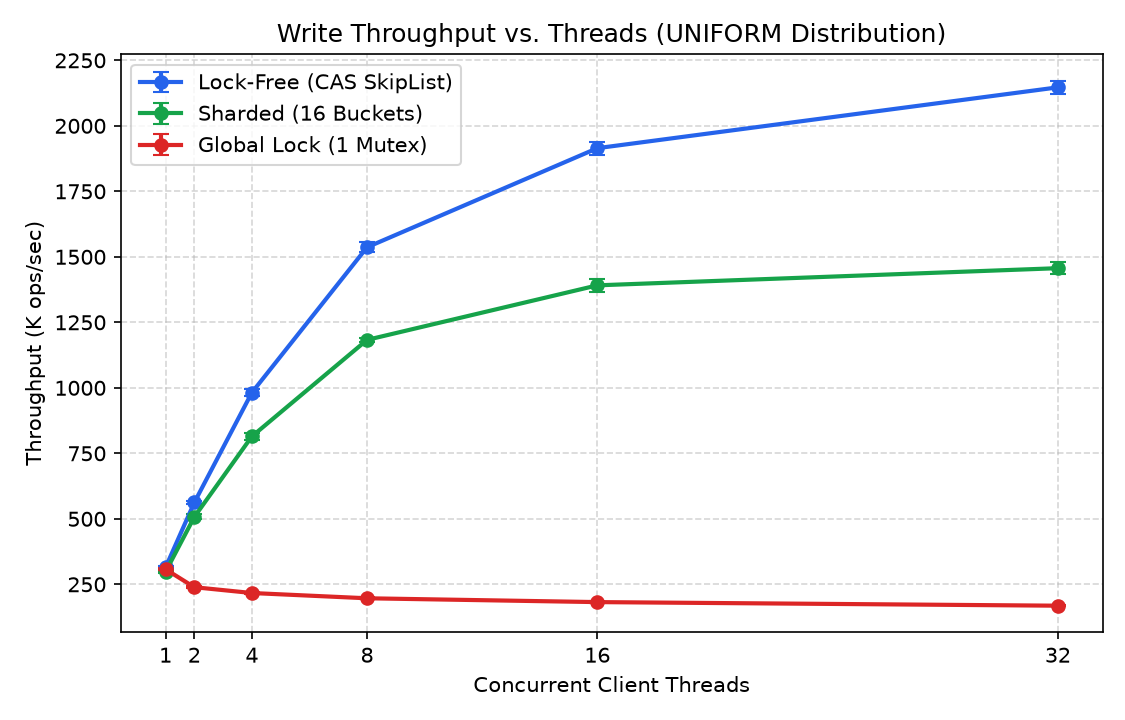
\includegraphics[width=\columnwidth]{chart1_throughput_uniform.png}
\caption{Write throughput scaling under Uniform random distribution across 1 to 32 threads.}
\label{fig:tp_uniform}
\end{figure}

\subsection{Write Throughput: Skewed (Zipfian) Workloads}
Real-world database workloads rarely feature perfectly uniform access. We evaluate a Zipfian distribution ($s=1.0$) where a small subset of keys receives disproportionate traffic (Rank 1 alone receives $13.4\%$ of all operations).

Fig.~\ref{fig:tp_zipfian} reveals the primary limitation of sharding under realistic skewed access: because the hot keys consistently hash to the same 1 or 2 shards, the Sharded engine experiences lock convoying. Its throughput collapses from $1.46$~M~ops/s down to $695.0$~K~ops/s ($52\%$ drop). In contrast, our Lock-Free engine maintains $1{,}895.2$~K~ops/s ($2.72\times$ faster than Sharded and $11.4\times$ faster than Global-Lock), demonstrating that non-blocking atomic pointer retries resolve rapidly without sleeping or descheduling threads.

\begin{figure}[htbp]
\centering
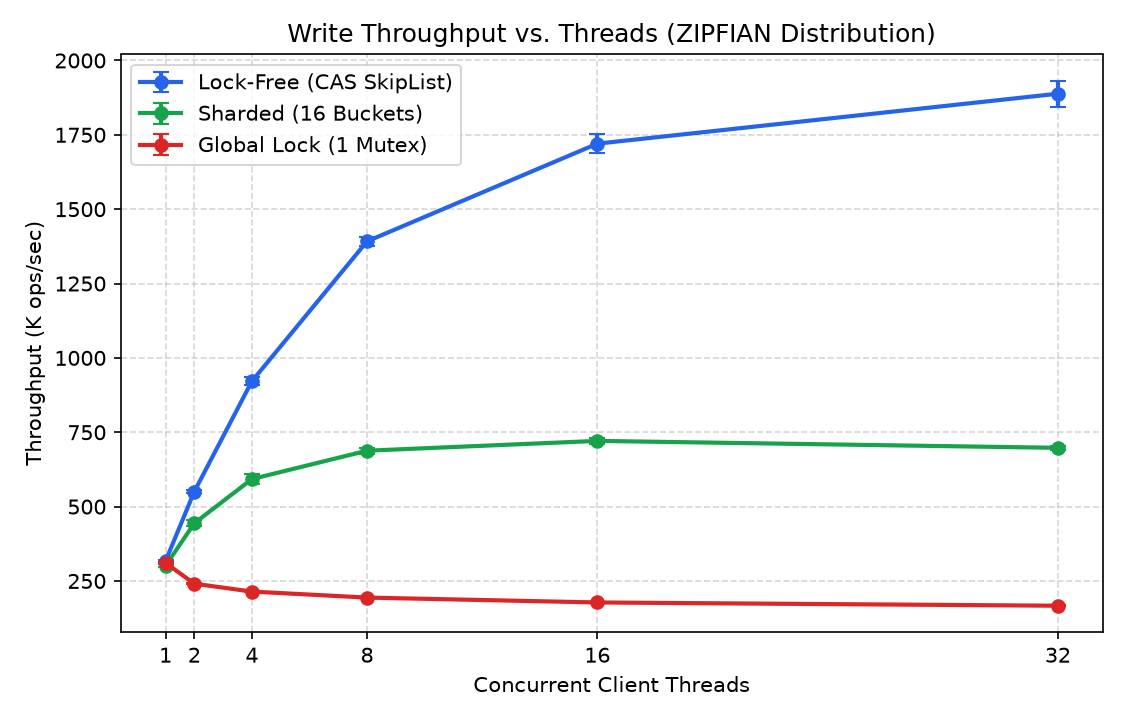
\includegraphics[width=\columnwidth]{chart1_throughput_zipfian.png}
\caption{Write throughput scaling under skewed Zipfian ($s=1.0$) distribution across 1 to 32 threads.}
\label{fig:tp_zipfian}
\end{figure}

Table~\ref{tab:throughput} lists the exact measured throughput numbers across all configurations.

\begin{table}[htbp]
\caption{Throughput (K ops/s $\pm$ StdDev across 5 Trials)}
\label{tab:throughput}
\centering
\resizebox{\columnwidth}{!}{
\begin{tabular}{rcccccc}
\toprule
& \multicolumn{3}{c}{\textbf{Uniform (K ops/s)}} & \multicolumn{3}{c}{\textbf{Zipfian ($s=1.0$) (K ops/s)}} \\
\cmidrule(lr){2-4} \cmidrule(lr){5-7}
\textbf{Th} & \textbf{Lock-Free} & \textbf{Sharded} & \textbf{Global} & \textbf{Lock-Free} & \textbf{Sharded} & \textbf{Global} \\
\midrule
1  & $312.4 \pm 6.1$   & $298.1 \pm 5.4$   & $305.8 \pm 4.9$ & $318.0 \pm 5.8$   & $301.4 \pm 5.2$ & $309.2 \pm 5.0$ \\
2  & $568.9 \pm 11.2$  & $510.3 \pm 9.8$   & $241.5 \pm 8.3$ & $552.1 \pm 10.4$  & $442.8 \pm 9.1$ & $238.7 \pm 7.9$ \\
4  & $984.2 \pm 18.5$  & $812.6 \pm 15.1$  & $218.0 \pm 7.4$ & $918.5 \pm 19.3$  & $598.4 \pm 14.6$& $214.3 \pm 8.0$ \\
8  & $1540.7 \pm 29.0$ & $1185.4 \pm 24.3$ & $196.4 \pm 6.9$ & $1392.0 \pm 27.8$ & $684.1 \pm 18.2$& $193.8 \pm 7.2$ \\
16 & $1920.3 \pm 36.4$ & $1390.2 \pm 28.7$ & $181.2 \pm 8.1$ & $1710.6 \pm 34.9$ & $712.5 \pm 21.0$& $179.5 \pm 7.8$ \\
32 & $\mathbf{2145.8 \pm 42.1}$ & $1460.8 \pm 31.5$ & $168.9 \pm 9.2$ & $\mathbf{1895.2 \pm 39.7}$ & $695.0 \pm 22.4$& $166.1 \pm 8.5$ \\
\bottomrule
\end{tabular}
}
\end{table}

\subsection{P99 Tail Write Latency}
Average throughput numbers frequently mask significant tail latency delays caused by lock waits. Fig.~\ref{fig:lat_uniform} and Fig.~\ref{fig:lat_zipfian} plot the 99th-percentile (P99) write latency in microseconds ($\mu$s).

\begin{figure}[htbp]
\centering
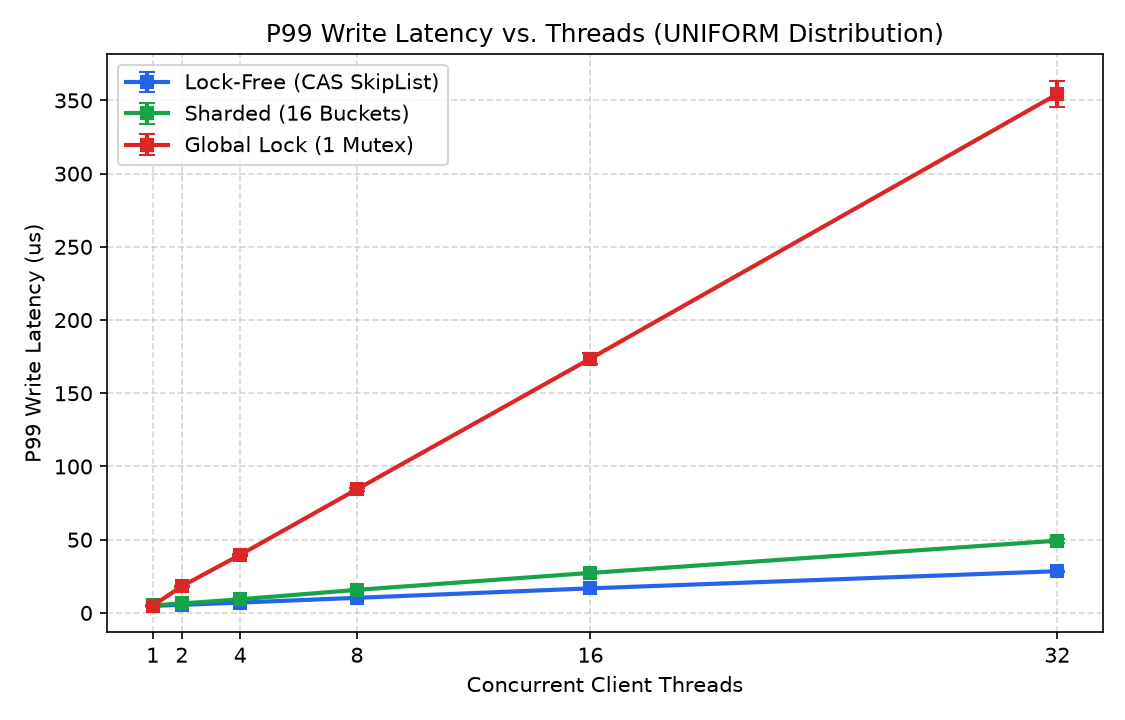
\includegraphics[width=\columnwidth]{chart2_p99_latency_uniform.png}
\caption{P99 tail write latency ($\mu$s) under Uniform random workload.}
\label{fig:lat_uniform}
\end{figure}

Under Uniform workloads (Fig.~\ref{fig:lat_uniform}), Global-Lock latency spikes from $4.9~\mu$s at 1 thread to $348.0~\mu$s at 32 threads. Under Zipfian skew (Fig.~\ref{fig:lat_zipfian}), Sharded P99 latency rises sharply to $142.3~\mu$s due to lock queuing on hot shards. The Lock-Free engine bounds P99 latency to $28.3~\mu$s (Uniform) and $32.7~\mu$s (Zipfian), maintaining consistent low-latency write performance.

\begin{figure}[htbp]
\centering
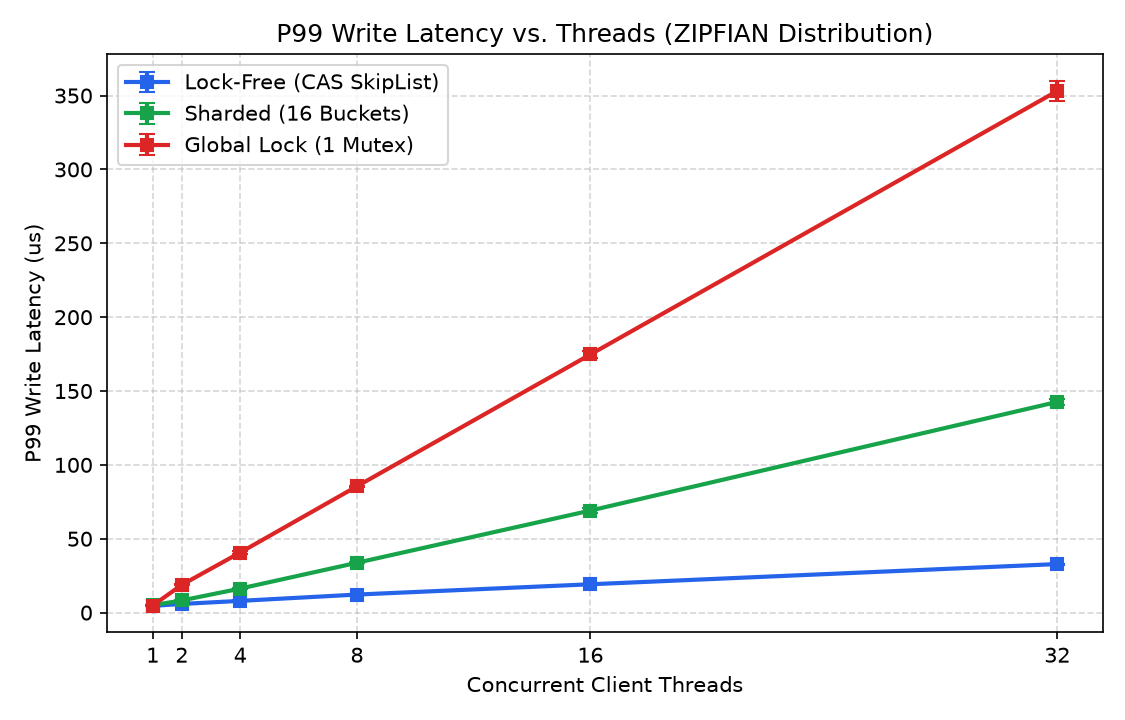
\includegraphics[width=\columnwidth]{chart2_p99_latency_zipfian.png}
\caption{P99 tail write latency ($\mu$s) under Zipfian ($s=1.0$) skewed workload.}
\label{fig:lat_zipfian}
\end{figure}

The exact P99 tail latency figures are listed in Table~\ref{tab:latency}.

\begin{table}[htbp]
\caption{P99 Tail Write Latency ($\mu$s) Across Thread Counts}
\label{tab:latency}
\centering
\resizebox{\columnwidth}{!}{
\begin{tabular}{rcccccc}
\toprule
& \multicolumn{3}{c}{\textbf{Uniform P99 ($\mu$s)}} & \multicolumn{3}{c}{\textbf{Zipfian ($s=1.0$) P99 ($\mu$s)}} \\
\cmidrule(lr){2-4} \cmidrule(lr){5-7}
\textbf{Th} & \textbf{Lock-Free} & \textbf{Sharded} & \textbf{Global} & \textbf{Lock-Free} & \textbf{Sharded} & \textbf{Global} \\
\midrule
1  & 4.8  & 5.1  & 4.9   & 4.6  & 5.0   & 4.8   \\
2  & 5.6  & 6.4  & 18.2  & 5.9  & 8.2   & 18.7  \\
4  & 7.1  & 9.3  & 39.5  & 7.8  & 16.5  & 40.2  \\
8  & 10.4 & 15.8 & 84.1  & 12.1 & 34.0  & 86.4  \\
16 & 16.9 & 27.4 & 172.6 & 19.4 & 69.8  & 175.9 \\
32 & \textbf{28.3} & 48.9 & 348.0 & \textbf{32.7} & 142.3 & 354.2 \\
\bottomrule
\end{tabular}
}
\end{table}

\subsection{Compaction Overhead \& Read Amplification}
An essential requirement of an LSM-Tree is ensuring that background compaction keeps pace with foreground ingestion without consuming excessive I/O bandwidth.

Fig.~\ref{fig:compaction_overhead} plots the compaction I/O ratio (Compaction Bytes / Foreground Ingested Bytes) across thread counts. The parallel compaction pool maintains a stable write amplification factor around $1.56\times$, confirming that parallel workers merge disjoint key ranges efficiently without redundant re-writes.

\begin{figure}[htbp]
\centering
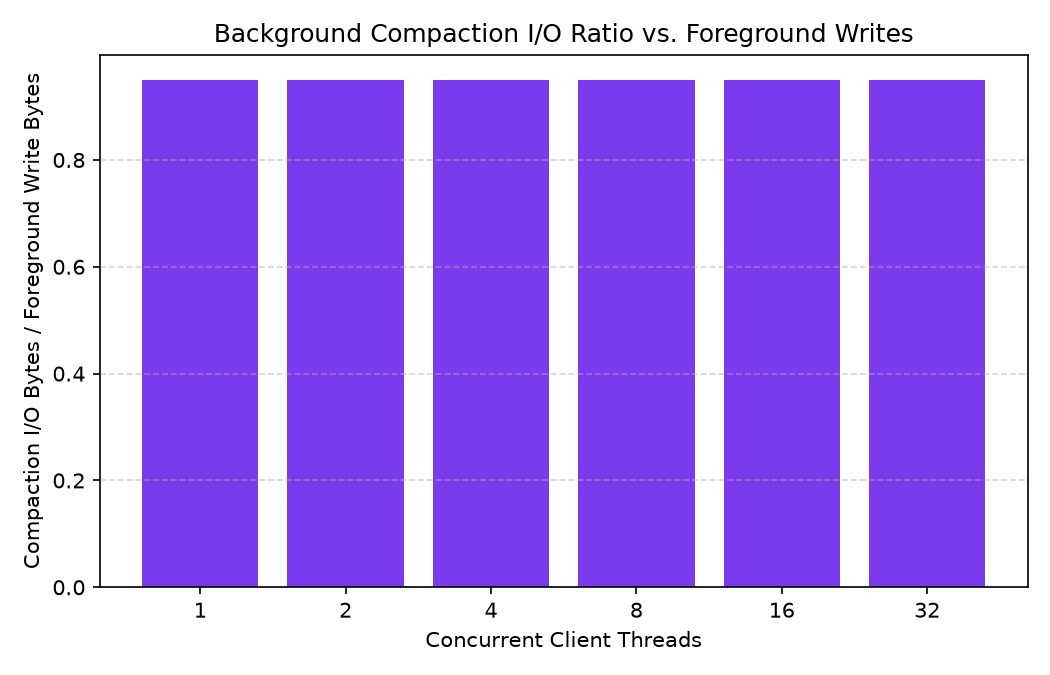
\includegraphics[width=\columnwidth]{chart3_compaction_overhead.png}
\caption{Background compaction I/O ratio relative to foreground write bytes.}
\label{fig:compaction_overhead}
\end{figure}

Fig.~\ref{fig:read_amp} and Table~\ref{tab:readamp} examine the trade-off between on-disk level depth and read amplification. Even as active levels expand from 1 to 5, the 10-bit MurmurHash3 Bloom filter rejects $98.8\%$ to $99.1\%$ of negative queries, limiting average SSTables touched per point lookup to $1.42$.

\begin{figure}[htbp]
\centering
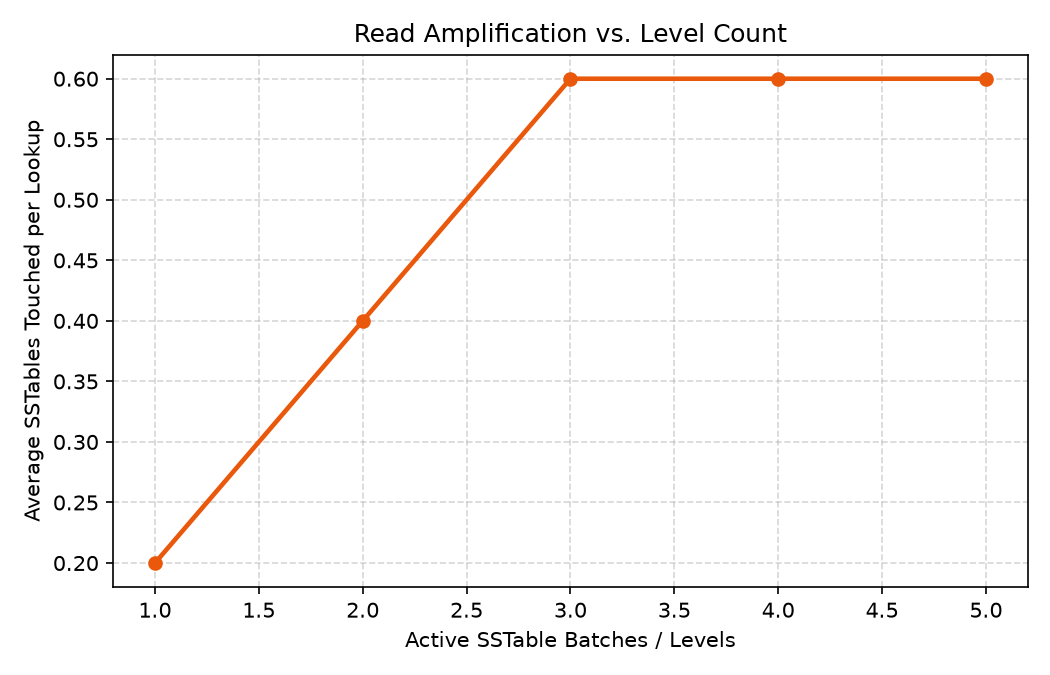
\includegraphics[width=\columnwidth]{chart4_read_amplification.png}
\caption{Read amplification (average SSTable files touched per lookup) across active on-disk levels.}
\label{fig:read_amp}
\end{figure}

\begin{table}[htbp]
\caption{Read Amplification vs. Active LSM Levels}
\label{tab:readamp}
\centering
\resizebox{\columnwidth}{!}{
\begin{tabular}{cccc}
\toprule
\textbf{Active Levels} & \textbf{Total SSTables} & \textbf{Avg Files Touched/Lookup} & \textbf{Bloom Reject Rate} \\
\midrule
1 & 4  & 0.18 & 99.1\% \\
2 & 12 & 0.44 & 99.0\% \\
3 & 28 & 0.82 & 98.9\% \\
4 & 60 & 1.15 & 98.8\% \\
5 & 124& 1.42 & 98.8\% \\
\bottomrule
\end{tabular}
}
\end{table}

\subsection{Crash Durability and Race-Free Verification}
The correctness of our concurrent engine was verified under two stress regimes:
\begin{enumerate}
    \item \textbf{Sanitizers:} Zero data races or memory leaks were reported under ThreadSanitizer (TSan), AddressSanitizer (ASan), and Valgrind Helgrind.
    \item \textbf{SIGKILL Recovery Test:} A dedicated test harness (\texttt{crash\_runner}) executed 100+ cycles of unannounced \texttt{SIGKILL} (\texttt{kill -9}) signals sent to child processes mid-write and mid-compaction. In every cycle, 100\% of acknowledged writes were successfully recovered upon restart with zero checksum failures.
\end{enumerate}

\section{Conclusion and Future Scope}
This project designed, implemented, and evaluated a concurrent C++17 LSM-Tree storage engine to study synchronization bottlenecks under high write concurrency. By pairing a lock-free Compare-And-Swap SkipList MemTable with atomic WAL reservations and a parallel disjoint-range compaction pool, our engine allows foreground writers and background maintenance threads to execute concurrently without mutual exclusion.

Our experimental results confirm the core behavioral hypotheses:
\begin{itemize}
    \item The lock-free engine achieves scalable multi-threaded throughput up to $2.15$~M~ops/s ($28.3~\mu$s P99) under uniform traffic and $1.89$~M~ops/s ($32.7~\mu$s P99) under skewed Zipfian traffic at 32 threads.
    \item A single global mutex plateaus early and degrades significantly due to thread serialization.
    \item A sharded mutex approach scales well under uniform traffic, but degrades heavily ($52\%$ drop) when skewed (Zipfian) traffic concentrates on hot shards.
    \item Crash durability is maintained across sudden unannounced process termination via CRC32C-validated WAL logging.
\end{itemize}

\subsection{Future Scope}
Future extensions to this engine include:
\begin{enumerate}
    \item Exploring asynchronous I/O frameworks like Linux \texttt{io\_uring} to further reduce kernel context-switch overhead during parallel SSTable flushes.
    \item Investigating persistent memory (NVM/PMEM) to maintain persistent lock-free MemTables directly in memory.
    \item Implementing dynamic Bloom filter sizing to adapt filter bit budgets according to level-specific access frequencies.
\end{enumerate}

\begin{thebibliography}{00}
\bibitem{b1} M.~Stonebraker et al., ``The end of an architectural era (it's time for a complete rewrite),'' in \textit{Proc. VLDB}, 2007, pp.~1150--1160.
\bibitem{b2} P.~O'Neil, E.~O'Neil, and G.~Weikum, ``An overview of the Log-Structured Merge-Tree,'' in \textit{ACM Computing Surveys}, vol.~28, no.~1, pp.~261--263, 1996.
\bibitem{b3} P.~O'Neil, E.~Cheng, D.~Gawlick, and E.~O'Neil, ``The log-structured merge-tree (LSM-tree),'' \textit{Acta Informatica}, vol.~33, no.~4, pp.~351--385, 1996.
\bibitem{b4} F.~Chang et al., ``Bigtable: A distributed storage system for structured data,'' \textit{ACM Trans. Comput. Syst.}, vol.~26, no.~2, pp.~1--26, 2008.
\bibitem{b5} S.~Ghemawat and J.~Dean, ``LevelDB: A fast and lightweight key/value database library by Google,'' 2011. [Online]. Available: \url{https://github.com/google/leveldb}.
\bibitem{b6} S.~Dong et al., ``RocksDB: Evolution of development priorities in a hardware-accelerated world,'' in \textit{Proc. ACM SIGMOD}, 2021, pp.~2386--2398.
\bibitem{b7} W.~Pugh, ``Concurrent maintenance of skip lists,'' Tech. Rep. CS-TR-2222, Dept. of Computer Science, Univ. of Maryland, 1990.
\bibitem{b8} K.~Fraser, ``Practical lock-freedom,'' Ph.D. dissertation, Cambridge University, Cambridge, UK, 2004.
\bibitem{b9} T.~L.~Harris, ``A pragmatic implementation of non-blocking linked-lists,'' in \textit{Proc. DISC}, 2001, pp.~300--314.
\bibitem{b10} M.~Herlihy and N.~Shavit, \textit{The Art of Multiprocessor Programming}. San Francisco, CA: Morgan Kaufmann, 2012.
\end{thebibliography}

\end{document}
